\documentclass[11pt]{article}
\usepackage[margin=1in]{geometry}
\usepackage{graphicx}
\usepackage{multirow}
\usepackage{multicol}
\usepackage{setspace}

\setlength\parindent{0pt}
\usepackage{hyperref}
\usepackage{amssymb,amsthm,amsmath, fancyhdr}
\pagestyle{fancy}

\usepackage{lipsum}

\begin{document}
\chead{Math 121 - Secant and Tangent lines, and the definition of a derivative}
\begin{enumerate}
    \item Write down the limit definition of the derivative. You can use Definition 4 from section 2.1, replacing $a$ with $x$.
    \item Use this definition to calculate the derivative of the following functions:
    \begin{itemize}
        \item $f(x) = 4x - 3x^2$
        \item $g(x) = x^2 - 3x +1$
        \item $y = \sqrt{x}$
    \end{itemize}
    \item Find the slope of the tangent line to each of the three curves above when $x = 1$.
    \item The distance travelled by a particle in a straight line is given by $$f(t) = t^2 - 8t + 18$$ where $t$ is in seconds. Compute the instantaneous velocity when $t = 4$. You can do this by finding the slope of the tangent line to the curve when $t = 4.$
    \item The graph of the function $g$ is below. Put the three values  $g'(-4)$, $g'(0)$, and $g'(2)$, in ascending order.\\
    \begin{center}
            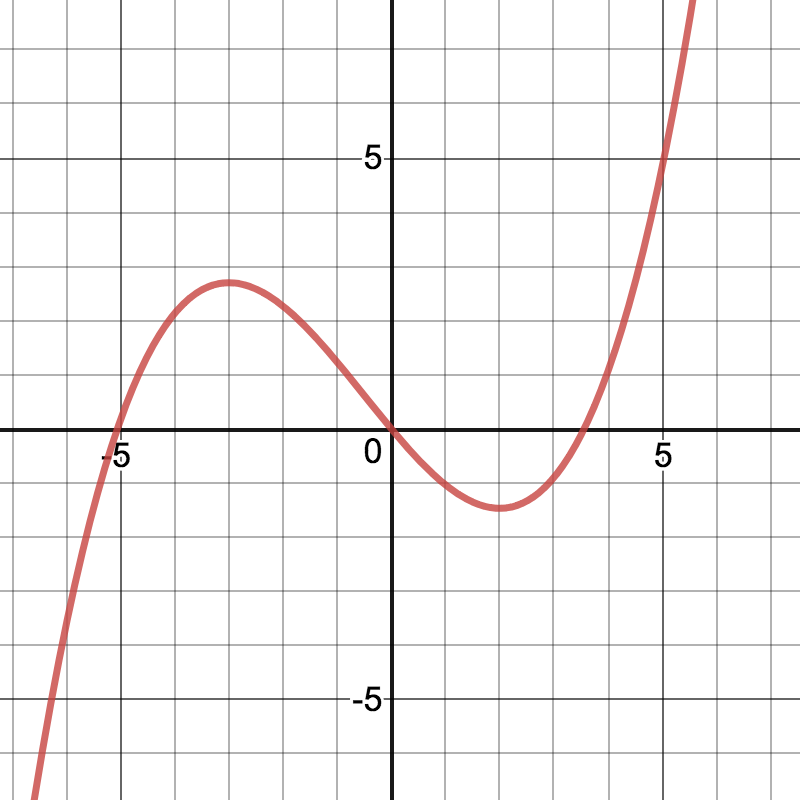
\includegraphics[width=0.5\textwidth]{1_4_graph}
    \end{center}
    \item (Bonus-style problem) Find the first derivative $\frac{dy}{dx}$ of the function $y = x^n$. You can assume $n$ is a positive integer.
\end{enumerate}
\end{document}